%%%%%%%%%%%%%%%%%%%%%%%%
% DO NOT TOUCH THIS PART
\documentclass{hitec}
\newcommand{\HT}{\textsc{\raisebox{0.1em}{h}\raisebox{-0.1em}{i}%
	\raisebox{0.1em}{t}\raisebox{-0.1em}{e}\raisebox{0.1em}{c} }}
	
\usepackage[table,xcdraw]{xcolor}
%%%%%%%%%%%%%%%%%%%%%%%%



% Enter the title of either the lab or some other title you think fits
\title{RGB LED Node}

% Place you team members here
\author{Andrew Hollabaugh}




\company{Rowan University}
\confidential{\textbf{-- ECE 09.321: Milestone 1 --}}


% Place the packages you want to use here.
\usepackage{hyperref} % This line is readily ommited of it makes trouble
\usepackage{graphicx}



\begin{document}
\maketitle
\section{Design Overview}
%As with normal lab reports, your application note should begin with an abstract talking about the overall experiment performed and what was achieved in the scope of this lab. Typically you want to limit this to about a paragraph, and you want to try to draw the reader into reading your work. Make sure you state the problem trying to be solved. You could also place an image of the project on this page if you want.

This project is an RGB LED controller that can be used in a network of similar devices to create an individually-addressable RGB LED strip. An MSP430G2553 processor is used, on the MSP430G2ET development board. Three PWM pins on the processor are used for each channel of the RGB LED. UART serial communication is used for the nodes to receive commands.

\subsection{Design Features}

%Keep this almost to a bulleted list which covers the features which you are showing off in your product. You can edit ``DesignFeatures.tex'' to add information to this section.
%\\
%\\
%These are the design features:
\begin{itemize}
    \item Three output channels to output to three LEDs or one RGB LED
    \item Independently controllable output channels
    \item Communication to other nodes over UART
\end{itemize}




\subsection{Featured Applications}


\begin{itemize}
    \item RGB LED strip
    \item Array of RGB lighting fixtures
    \item Sending visual information
\end{itemize}




\subsection{Design Resources}

%This is just a quick link to the code and design folders you generated during the product. Make sure to actually make the links live.

\href{https://github.com/Intro-To-Embedded-Systems-RU09342/milestone-1-andrewhollabaugh}{Link to Github page}





\subsection{Block Diagram}

%As it sounds, this is just a block diagram of how the system is connected. The block diagram should be designed in such a way that other than the Figure Caption saying something like ``System Block Diagram'', it should be able to be understood what is going on.

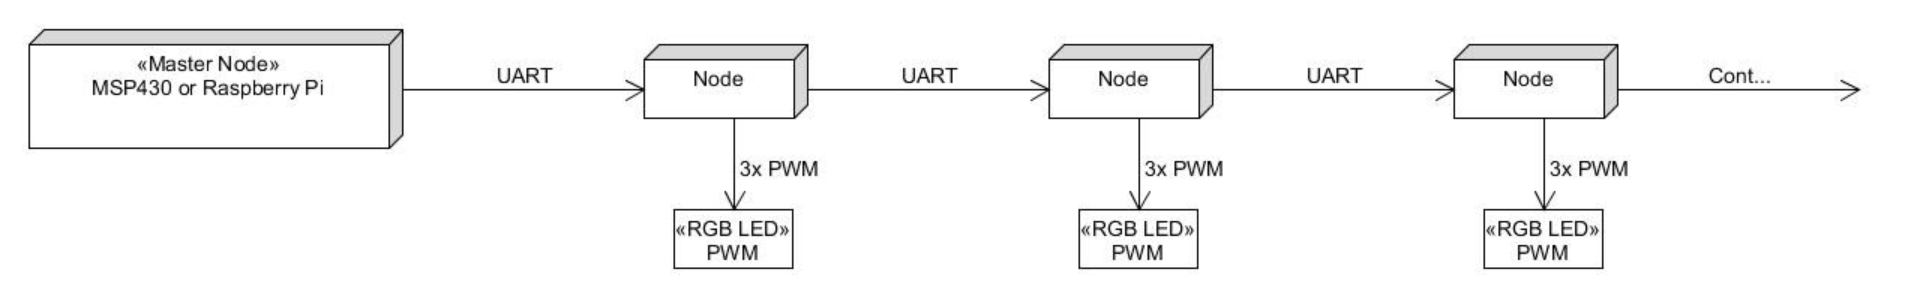
\includegraphics[scale=0.4]{block-diagram.png}
Figure 1: System Block Diagram




\subsection{Board Image}

%You need to include either a picture of the PCB you have designed or a clear picture of the breadboard which you constructed.

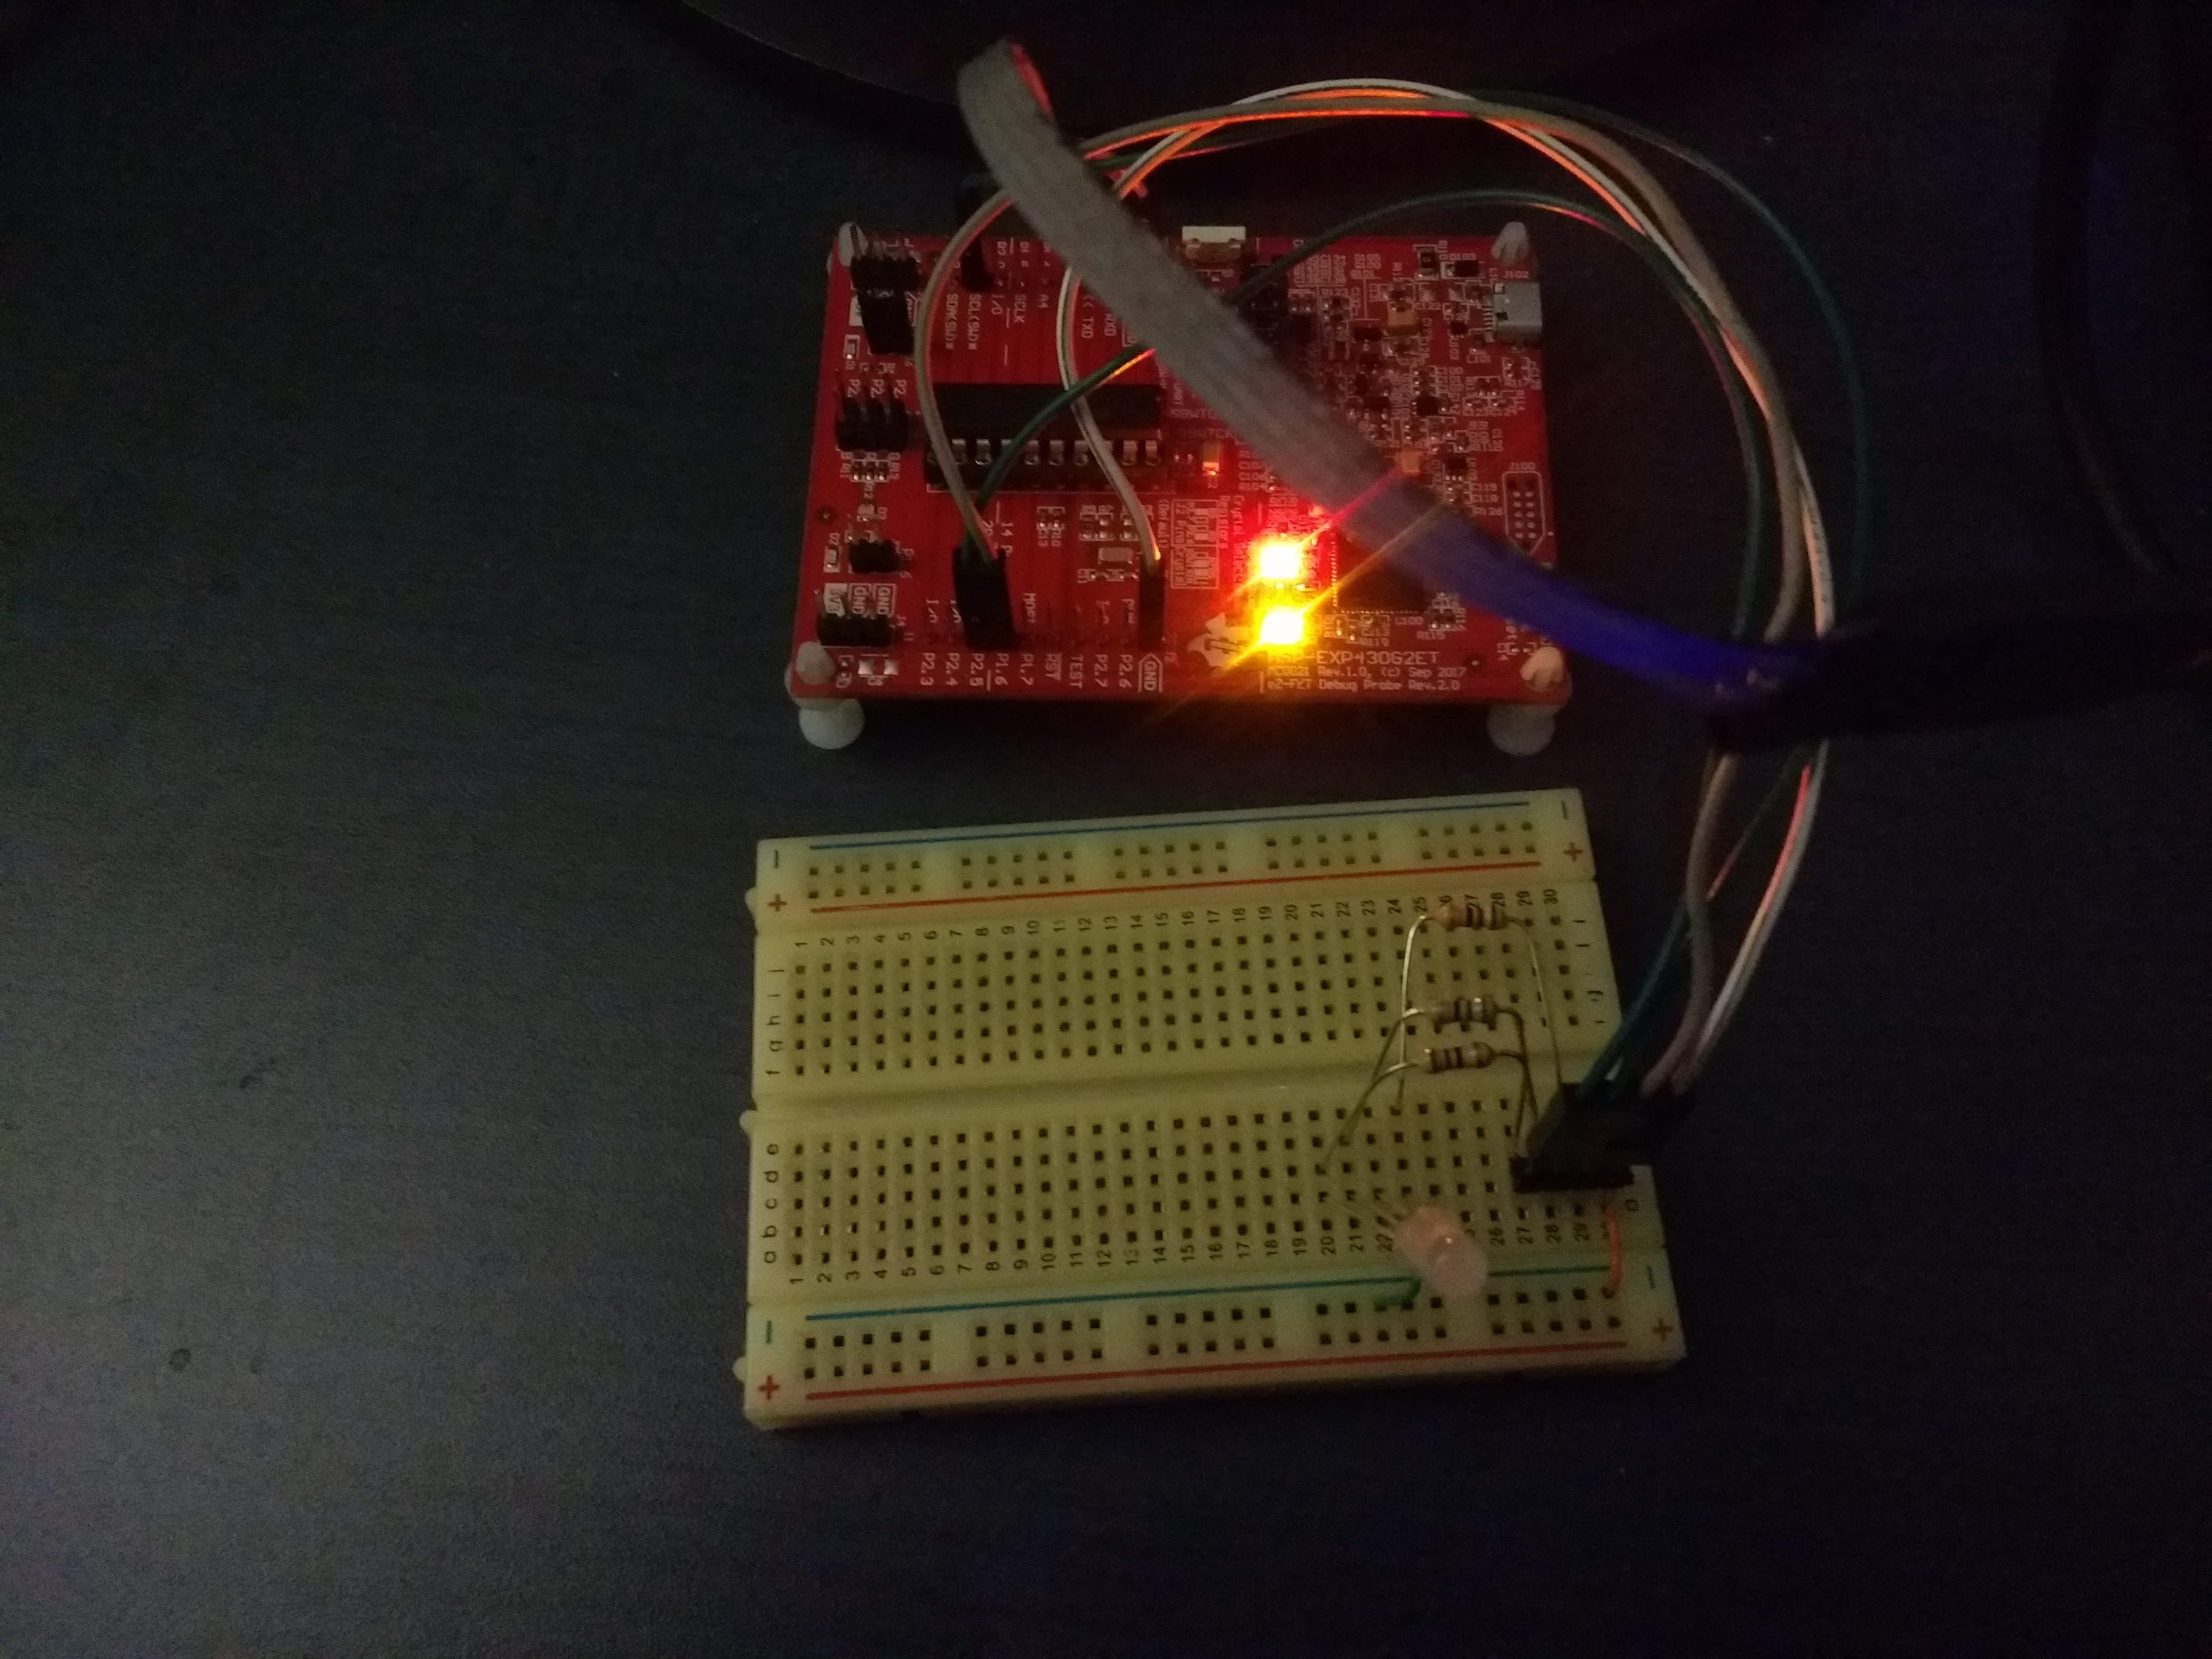
\includegraphics[scale=0.1]{board-image.jpg}
Figure 2: Picture of Breadboard and Dev Board




\section{Key System Specifications}

You can organize these as a table. This is meant to talk about the specifications which your system is capable of performing. I highly recommend looking up a \LaTeX table generator online.

\begin{table}[]
\begin{tabular}{|c|c|c|}
\hline
\rowcolor[HTML]{C0C0C0} 
\textbf{PARAMETER} & \textbf{SPECIFICATIONS} & \textbf{DETAILS}                                                                                      \\ \hline
Communication        & UART (serial)       & \begin{tabular}[l]{@{}c@{}}UART Serial communication is used with 8 data bits, \\1 stop bit, and 9600 baud rate. A stream of bytes is \\received, some of the bytes are used to control\\ the brightness of the leds, then it transmits the rest of the \\data to the next node.\end{tabular} \\ \hline
LED Channels        & 3                    & \begin{tabular}[c]{@{}c@{}}The LED output channels go to each color\\ of the RGB led (red, green, and blue). \\Other colors could also be used.\end{tabular} \\ \hline
\end{tabular}
\end{table}




\section{System Description}

%Use this section to introduce the system as a whole and introduce a problem which you are trying to solve. Normally this is like a paragraph long to introduce a problem, but for the first milestone, there is not that much you can talk about.

This device allows individual nodes in a network, to be configured independently. By using RGB LEDs, a network of these nodes create a string of LEDs whose colors can be independely configured.




\subsection{Detailed Block Diagram}

%The main difference here between the previous block diagram is the level of detail. This should show specific pins on the device and voltage levels. Don't go so far as putting in pictures of how the peripherals are connected to each other inside of the controller, but enough that you could basically put this thing together again.

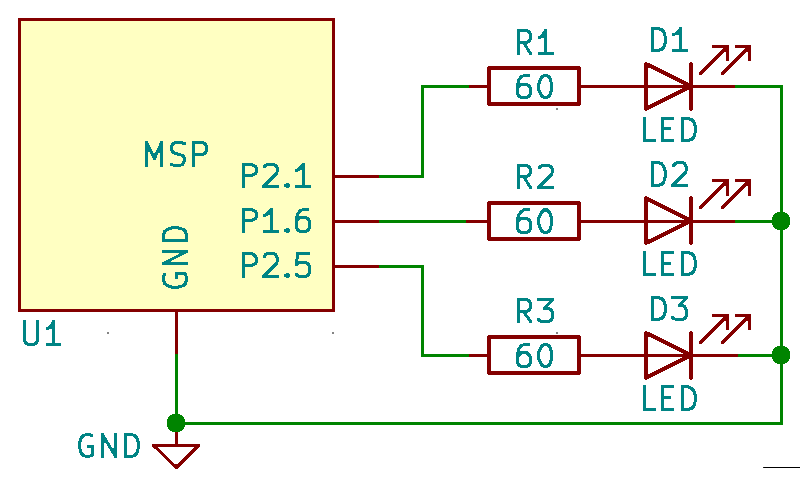
\includegraphics[scale=0.3]{detailed-block-diagram.png}

Figure 3: Detailed Block Diagram




\subsection{Highlighted Devices}

%This just needs to be a bulleted list of what parts you used (not including passive components) with just a quick blurb of what it is doing in your system.
\begin{itemize}
    \item MSP430G2553 processor (on MSP430G2ET development board): processes serial data and creates PWM signal for LEDs
    \item RGB LED: lights up in a combination of the three primary colors (red, green, and blue) corresponding to the PWM signals received from the MSP
    \item USB-to-serial cable: contains FTDI chip that allows the USB port of a computer to communicate with the MSP's UART interface
\end{itemize}




\subsection{Device/IC 1}

%You want to focus on each IC or block in your subsystem. So for Milestone 1, you might want to first talk about the procesor, and then in the next section talk about the LED and the driving circuitry. For each one of these, you actually should get pretty technical and aim for about a paragraph.

The MSP430G2553 is a 16-bit, RISC-based microcontroller. In this project, it operates at 3.3V and has a clock frequency of 1 MHz. This processor is a good choice due to its low power consumption and its UART and PWM output capabilities. This device receives a string of bytes over UART, and interprets the string as a set of commands. It picks out the values for the three LED brightnesses, then sends the rest of the data to the next node. One the brightness values are known, it outputs three PWM signals, one for each LED channel, to the LEDs. The duty cycle of the wave, which determines the channel's brightness, is determined by an 8-bit value in transmission it receives.




\subsection{Device/IC 2}

The RGB LED contains three single-color LEDs, one for each primary color (red, green and blue). Therefore, it can be viewed as three separate LEDs for simplicity. The RGB LED has four pins: one is ground, and the other three are positive voltages for each LED. The LEDs are connected to the MSP430 via digital PWM output pins and a series resistor. The series resistors were calculated to be 60 Ohms, using the forward voltages of the LEDs.





\section{SYSTEM DESIGN THEORY}

%This section and its subsections I want to see you really talk about what you have done with the project. You should talk about the overall operation of the system pointing out what each IC or component is responsible for (again, except for passive, unless they are interesting). Set yourself up for the following sections by making it clear what the major part of the systems are.

The program running on the MSP430 does two major things: interpret and send serial commands, and output PWM signals to the three LEDs.





\subsection{Serial Communication}

%For these design requirements, really dig into the technical grit. This is where you have to explain what you did as the engineer to meet the system requirements.

The serial communication protocol used is UART (Universal Asynchronous Receiver Transmitter). This protocol allows for easy tranmission of bytes. A standard protocol is used so the nodes can communicate effectively. This protocol can be any number of bytes long, and always starts with a byte containing the number of bytes in the entire transmission. The next three bytes are the brightness values for the first node's LEDs in the order of red, green, then blue. The next sequence of bytes is is the brightness values for next node's LEDs. Any number of multiples of three bytes can be added to this section to add commands for more nodes. The last byte of the transmission is always a newline (0x0d). In the way this protocol is interpreted by the program, the newline character is uncessesary. The program cannot use detecting newlines as a way to detect the end of the transmission, because 0x0d could be a brightness value. Instead, only the first byte (number of bytes in transmission) is used. The program keeps track of how many bytes have been processed to determine the end of the transmission accurately. The program uses an interrupt, which triggers when a UART character is received. When the interrupt is not being run, the system is doing nothing and is set to low-power mode 0 (LPM0).




\subsection{PWM Signals}

The MSP430 uses three PWM outputs to control the three LED channels. Timers are used to generate the PWM signals. The MSP430G2553 contains two TimerA peripherals, each of which has two PWM outputs. Two PWM outputs from TimerA1 are used, as well as one PWM output from TimerA2. The timers are set to UP mode, with SMCLK as the clock source. No prescaling is used for a high frequency output, resulting in a more constant brightness. The brightness values from the serial command are assigned to the capture/compare registers. The PWM signal is generated by comparing the value in the capture/compare register (the brightness value) with the current timer value. This comparison between a horizontal line and a triangle wave results in a square wave, the PWM signal. Pins P1.6, P2.1, and P2.5 are used for PWM output. Only certain pins can be used, since only certain pins are connected to the PWM-generating hardware.




\section{Getting Started/How to use the device}

%This section is all about actually using and interfacing with your device. Write this as if you were to hand your system to someone and they needed to get the thing working.

Connect the LED and resistors on a breadboard according to Figure 3.
\\
Interfacing this device with a computer involves using a USB-to-serial cable. Connect the +5V, GND, RX, and TX on the UART side of the USB-to-serial cable to the corresponding pins on the MSP430. Connect the USB end to a computer.



%\textbf{NOTE:} You will be choosing what subsections to include in here. I highly recommend looking at other examples from TI and other companies to see how they break up there documents.

\section{Getting Started Software/Firmware}

%Let this section specifically deal with the firmware and software for your project and how to interface with it. Again, look at other documents to get a sense for what is contained here. Below are some example sections you could consider using.

The code needs to be compiled using msp-gcc. MSP430Flasher is a good tool for flashing the chip.



\subsection{Hierarchy Chart}

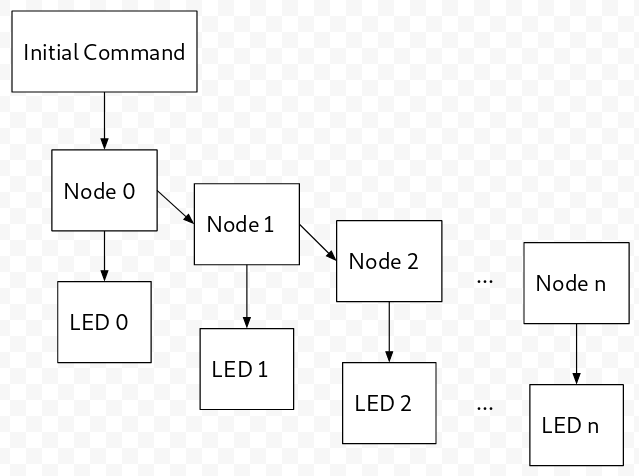
\includegraphics[scale=0.5]{hierarchical-diagram.png}

\subsection{Communicating with the Device}

Use a serial terminal to communicate with the node. First it must be connected using a USB-to-serial cable. Ensure the serial terminal is set to 9600 baud rate, and 8 data bits and 1 stop bit. Data is sent in the following format: first byte is number of total bytes in transmission, next three bytes are the R, G, and B values for the first node, the next any number of bytes (in multiples of three) is the R, G, and B values for nodes further down the line, and the last byte is a newline (0x0d).

\section{Test Setup}
Ensure the program is flashed onto the MSP430. Use a breadboard to connect the RGB LED to the three resistors. Use jumper cables to connect to the three pins on the MSP430. Use a USB-to-serial cable to connect the MSP430's UART to a computer. Use a serial terminal to connect to the processor, such as CuteCom, minicom, RealTerm, putty, etc. Send an example command, such as 05ffffff0d. This should set all three LEDs to full brightness, making the RGB LED appear white in its full brightness. To connect more nodes, connect the TX pin of the first node to the RX pin of the second. Also ensure they are both powered. Any hex values after the first four will specify brightnesses for the second node.

%\subsection{Test Data}

\section{Design Files}

\subsection{Schematics}

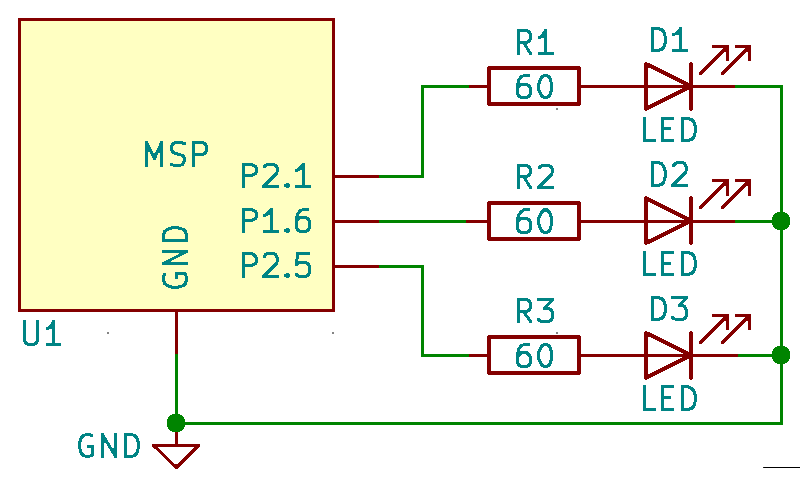
\includegraphics[scale=0.3]{detailed-block-diagram.png}

\subsection{Bill of Materials}
\begin{itemize}
    \item MSP430G2553
    \item RGB LED
    \item 60 ohm, 1/4 watt resistor (3)
\end{itemize}

%\subsection{Layout Prints (if applicable)}

%\subsection{Diptrace Project (if applicable)}

%\subsection{Gerber Files (if applicable)}

%\subsection{Assembly Drawings (if applicable)}

\end{document}

